\setmainfont{Noto Serif}
\setsansfont{Noto Sans}
\setmonofont{Noto Sans Mono}
\setstretch{1.35}

\section{ЭПР спектроскопия}
1С. Постройте спектр ЭПР катион-радикала дурола.
\par
\begin{wrapfigure}{r}{20mm} %this figure will be at the right
   \centering
    \vspace{-3.6ex}
    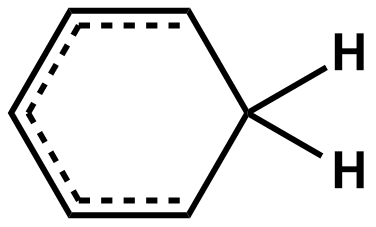
\includegraphics[width=15mm]{images/Fig_2_7_1.png}
    \vspace{-4ex}
\end{wrapfigure}
2С. Постройте спектр ЭПР радикала, структура которого изображена на рисунке. Константа СТВ с $\beta$-протонами в данном радикале равна 4,5~мТл.
\par
3К. Определите процентное содержание изотопа $^{13}\text{C}$ в метильном радикале, если соотношение интенсивностей трех высокопольных линий в спектре ЭПР данного радикала равно 1:3:3, начиная с самой высокопольной. Константа СТВ с ядром $^{13}\text{C}$ равна 40 Гс.
\par
4С. Постройте спектр ЭПР для радикала $\text{NH}_2^{\boldsymbol{\cdot}}$. Константы сверхтонкого взаимодействия равны: $a_{\text{N}}$ = 10 Гс, $a_{\text{H}}$ = 24 Гс. Как изменится спектр, если один атом водорода заменить на дейтерий?
\par
5С. Какая температура необходима, чтобы ориентировать 75\% спинов некоторого радикала в магнитном поле 1 Тл?
\par
6С. Нарисуйте спектр ЭПР во втором порядке теории возмущений для следующих радикалов: $\text{H}$, $\text{H}_2^{\boldsymbol{\cdot}}$, $\text{D}$, $^{\boldsymbol{\cdot}}\text{CH}_3$.
\par
7С. Нарисуйте спектр ЭПР $\text{D}_2^{+\boldsymbol{\cdot}}$ при $T \rightarrow$ 0 К.
\par
8. В рамках теории возмущений второго порядка рассчитайте как будет выглядеть спектр ЭПР иона ванадила, если $a$ = 100 Гс, $g$ = 2, $I$ = 7/2, $\nu$ = 9000 МГц.
\par
9К. Метильный радикал стабилизировали в некоторой дейтерированной матрице. С течением времени произошел обмен атомов водорода радикала и~дейтерия матрицы. Постройте ЭПР спектр эквимолярной смеси $^{\boldsymbol{\cdot}}\text{CHD}_2$ и $^{\boldsymbol{\cdot}}\text{CH}_2\text{D}$ радикалов. Укажите, сравнивая относительные интенсивности каких линий, возможно определить содержание данных радикалов в смеси.
\par
\begin{wrapfigure}{r}{20mm} %this figure will be at the right
   \centering
    \vspace{0.55ex}
    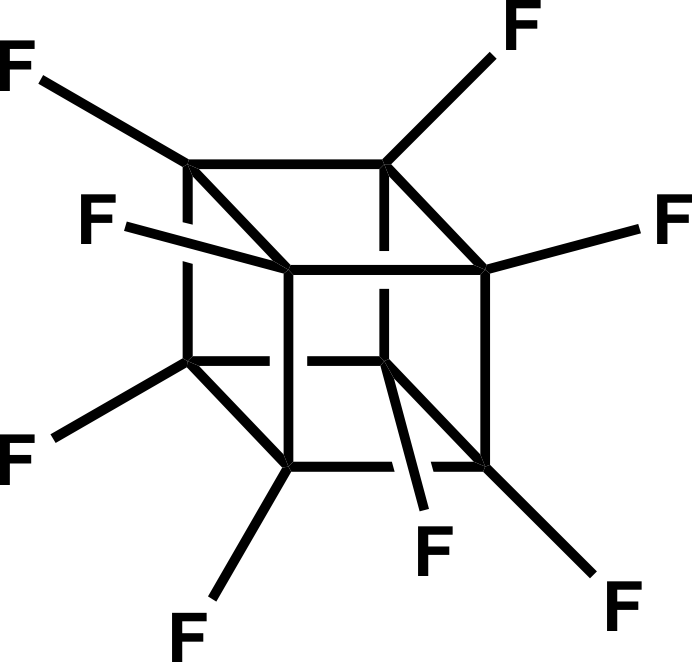
\includegraphics[width=20mm]{images/Fig_2_7_10.png}
    \vspace{-3ex}
\end{wrapfigure}
10К. Фторированные аналоги полиэдрических углеводородов локализуют электрон внутри полости своего каркаса при их восстановлении. В 2022 году японским химикам удалось синтезировать перфторкубан и стабилизировать его анион-радикал, полученный в результате $\gamma$-облучения, в матрице гексаметилэтана при 77 К. Нарисуйте спектр ЭПР данного анион-радикала с учетом второго порядка теории возмущений. Считайте, что неспаренный электрон локализован в каркасе перфторкубана, а константа СТВ на ядрах фтора равна 196,2 Гс.
\par
\begin{wrapfigure}{r}{25mm} %this figure will be at the right
   \centering
    \vspace{-4ex}
    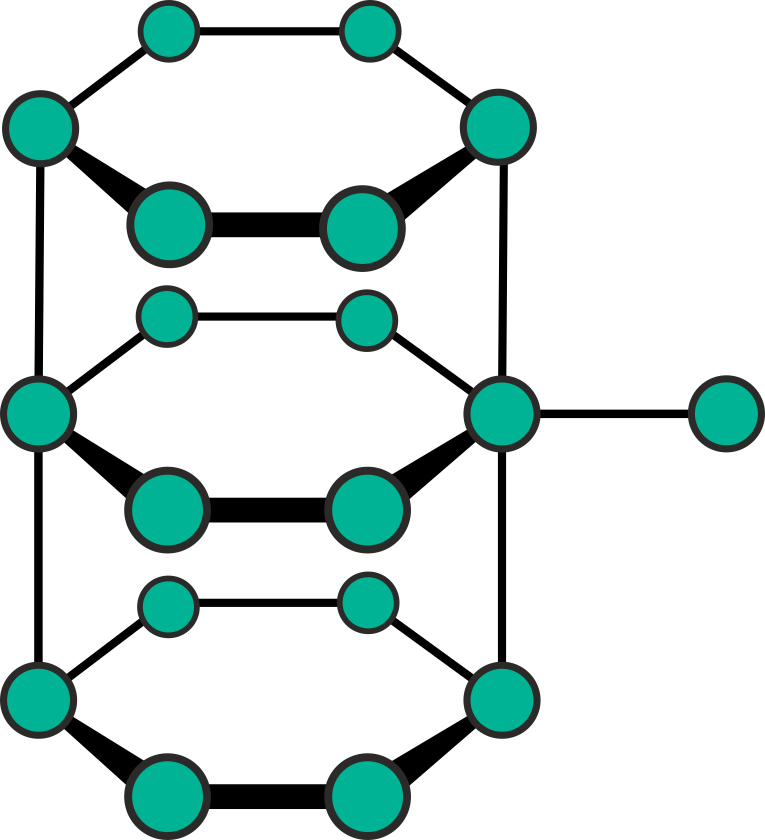
\includegraphics[width=14mm]{images/Fig_2_7_12.png}
    \vspace{-4ex}
\end{wrapfigure}
11C. Для хюккелевской системы, структура которой изображена на рисунке, постройте спектр ЭПР. Определите количество линий в~этом спектре и их относительную интенсивность.
\par
12С. Постройте спектр ЭПР для радикала $\text{H}_2^{+ \boldsymbol{\cdot}}$ в нулевом внешнем магнитном поле и $T$ $\rightarrow$ 0 К.
\par
13С. Построить спектры ЭПР радикала $\text{CF}_3$ с константой СТВ $a_{\text{F}}$ = 142 Гс и радикала $^{13}\text{CF}_3$ с константами СТВ $a_{\text{F}}$ = 142 Гс, $a_{^{13}\text{C}}$ = 272 Гс с учетом второго порядка теории возмущений.
\par
